\chapter{Methodology}
\label{chap:meth}

This chapter starts with the analysis of requirements for implemented software.
After that, the implementation is discussed in more detail in the dedicated
section.

\section {Requirements analysis}

As previous chapters of this paper suggest, the goal of this paper is to create
an implementation of a TCP/IP stack suitable for a persistent system. In
particular, I use a port of Phantom OS to Genode OS framework as a target
platform.

This section contains a list of requirements that a developer of such a stack
should take into account when implementing their own port.

\subsection {Transparent peer disappearance}
One of the fields in which persistent systems are actively applied is IoT. In an
intermittently powered environment, a system that can efficiently restore its
state is preferable to a system that experiences a booting process that consumes 
a lot of energy.

In such cases, hosts can experience long downtimes. Standard TCP implementations
are not applicable here because they perform retransmission of packets for only
a limited amount of time, and then close connection.

To make the development of stable persistent applications easier a temporary 
shutdown should be transparent for the client app. That means that the network 
connections state should be the same when the powered-off host restarts.
To achieve that persistent TCP implementation should either (1) backup and
restore connections state or (2) make the disappearance of the remote peer
invisible for application on the other end of the connection.

\subsection {Rollbacks}

The technique used in Phantom OS to provide persistence is memory snapshots of 
PVM memory space. They are taken in a live mode so that processes inside the VM
continue to run. Then, when power is back on, the latest snapshot is restored by
copying it to the main memory. The part of Phantom that is outside of VM is
assumed to be stateless in the usual case, which is not the case in Genode port.
That is why snapshotting and restoring of Genode part of the system is done with
callbacks, which accept and provide blobs of data to be saved in persistent 
memory. 

In the case of the intermittently powered Phantom system, this can cause
trouble, when clients actively use networking. While the system performs a
snapshot, the TCP stack can still proceed with receiving data. In this case,
TCP on receiving side will acknowledge packets, as protocol prescribes.
The issue is that acknowledged packets are getting deleted from the
retransmission queue, and therefore not present at the sending site. However,
they are not present in the snapshot on the receiver's side. In this case, after
the snapshot is used to restore the state of the receiver, the receiver will
request the packet (with duplicated ACK) that the sender is unable to 
retransmit. In this case, the sender's TCP will respond with RST and then close
the connection.

Three solutions exist that may solve the problem above. One is to forbid
sending acknowledgment packets if a received packet is not included in any
snapshot. However, this will either dramatically increase the number of
retransmissions in a network, which will result in reduced network performance
or it will require doing snapshots very often. In such a case snapshot should
be performed each 50ms. With a snapshot duration of around 10 seconds, this is
not acceptable.  

The other solution is to keep a buffer in a persistent memory that will store
all packets that a user of TCP had not consumed yet. In this case, persistent
memory can be a regular file or memory space that will fall into a snapshot for
sure.

The third approach is to have a dedicated broker inside a network that will
function similarly to the buffer in the second case. The broker can save all
acknowledged packets in a network, and flush its queue when it detects that
receiving host has done a snapshot. ICMP messages or some similar mechanism
will be useful to notify the broker about the end of the snapshot process.

\subsection {Compatibility with existing protocols}

The third design goal is not directly related to providing persistent I/O
abstraction to the clients of a network stack. Since snapshotting is a very
popular technique for implementing persistent systems, and Genode is actively
used to develop various operating systems, it is probable that some other
developers might want to use persistent TCP in their software.

That means that result of this work should be a standalone application that
works without Phantom and is flexible enough to support all use cases that may
arise. Fortunately, Genode's component-based architecture helps greatly with
it.

Another thing that should be addressed in the design of the API of the system,
is easy migration from non-persistent TCP stacks already available in Genode,
namely lwip and lxip. To do this I intend to design API very similar to regular
sockets or even exactly the same, but with different call semantics. I also
plan to add a Virtual File System (VFS) plugin that will expose sockets as
regular files because this is the way how Genode developers suggest
integrating sockets into the Genode ecosystem since version 18.11. With such
implementation, even relinking of existing binary will be not needed. The only
thing user would need is to change the configuration of the init Genode
component.

\section{Implementation process}

I have chosen to implement a persistent TCP stack in form of a Genode component
that will serve as a plugin for a VFS. The users of the TCP stack should add
signal handlers to their components for signals of type SIG\_SNAP and
SIG\_RESTORE. When SIG\_SNAP is received, it is passed to the persistent TCP VFS
plugin which gathers data that should be saved into persistent memory and calls
filesystem service to save socket snapshot structure into persistent memory.

Symmetrically, when SIG\_RESTORE is received, the component will access the
previously saved file and read information about sockets state at the snapshot
moment.

The exact structure of the data needed for the connection restore process and
some conditions for successful persistence of sockets will be discussed in the
following sections of this chapter.

\subsection{Snapshot structure}

As discussed earlier, I decided to make a TCP stack persistent using periodic
snapshotting.  To be useful in process of restoring the state, the snapshot
should indeed have some data stored in it. The content of the snapshot is
discussed in detail in this section.

When deciding about snapshot structure, two distinct approaches exist. The first one is to make a full-memory snapshot, saving each page of virtual
memory into persistent memory. To make snapshot consistent, all threads that use
these memory pages should be stopped, or writing to the pages should be
prohibited.  One of the disadvantages of this type of snapshot is that it is not userspace
friendly, since memory pages are usually managed in the kernel. The last
downside is its relatively big size, in terms of hundreds of megabytes. 

The second approach is to use selective snapshotting. In this case, when the
component forms a snapshot, it should first read certain set of state variables
from memory then serialize them together. After that, the serialized structure
is persisted. The benefits of this approach are easier implementation, and the
smaller size of the snapshot structure. The smaller snapshot size leads to the faster
snapshot/restore process.

I have chosen the second approach. Currently, Genode does not support
full-memory snapshotting, and implementing it from scratch is almost
impossible. Though it may be possible to mimic a full memory snapshot for a
single component by persisting all its dataspaces, it poses additional
challenges. For example, a dataspace might be shared with other components that
are not persisted. In this case persistent component expects its sibling to
write something to the dataspace they used for memory-mapped communication
earlier, and the sibling is unaware of any communications before power loss.

To snapshot socket state selectively, I needed to decide which data needs
to be saved. 

\begin{figure}
    \centering
    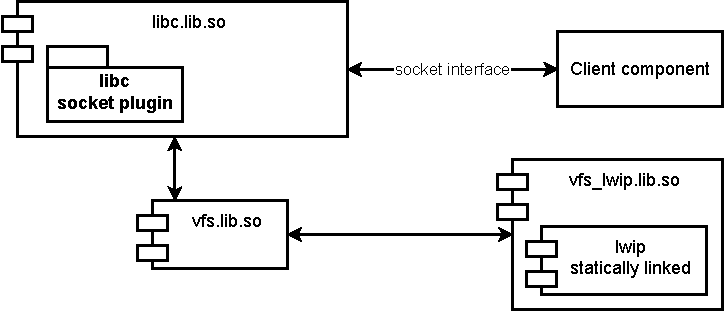
\includegraphics[]{figs/vfs_components.drawio.pdf}
    \caption{Control path of socket API}
    \label{fig:socket_via_vfs}
\end{figure}

Figure \ref{fig:socket_via_vfs} shows all libraries that are related to the
socket interface. To find out, which of them contain state that needs to be
snapshotted I have studied their source codes and how their clients should use
them. 

The libc is the library that provides a libc runtime and API for client
applications. Part of the standard libc API is a socket API. It includes
well-known functions socket(), bind(), listen(), and others. Genode libc
implementation is based upon a FreeBSD libc with some adjustments. In this
library socket API is implemented as a libc plugin. Libc plugin is a logically
independent part of code, responsible for a single API. In this case, it is
sockets API.  

Libc socket plugin maintains a single Socket\_fs::Context structure per each
created socket. This structure encapsulates a socket state variable \_state,
which is used to determine which calls on the socket are allowed in the current
state. The Context also has \_fd\_flags variable, which represents flags set on
socket. To make the behavior of the plugin consistent after restore, the \_state
and \_fd\_flags variables should be restored.

Internally the libc plugin uses VFS to provide its functionality. VFS is
implemented in form of a shared library, vfs.lib.so. This library is not
interesting from point of snapshotting, as it does not contain any state
itself.  The library in our case is just a proxy and a dynamic loader for VFS
plugins.

State of vfs\_lwip.lib.so should certainly be snapshotted, as this library
contains information required for operation of the TCP itself. Information is
stored in form of Protocol Control Blocks (PCBs). PCB is a structure used at a
protocol level that holds all the data needed for the protocol stack socket
uses. More details about PCBs can be found at \cite{stevens1996tcp}. Each
socket corresponds to exactly one PCB. Fortunately, it seems to be enough to
save the states of all PCBs and then restore them.

\subsection{Snapshot location}

The goal of this paper is to design a persistent networking stack suitable for
Phantom OS. Due to this, it is possible to include a snapshot of the TCP stack
into the Phantom VM snapshot structure. However, I decided that a persistent
network stack can be useful not only for the Phantom OS but also for other
persistent systems. These systems can use other mechanisms for persistence. Due
to this, I decided to make an abstract interface that has functions for saving
and loading binary data from persistent memory.

For simplicity, the only implementation of this service saves its state
directly to the hard drive volume attached to VM. An implementation that saves
and loads data using the Phantom snapshotting mechanism is currently in
progress.

/subsection{Approach with memory}
As a first approach I tried to save memory pages that belong to network stack and 
restore them on booting. At first I tried to snapshot the whole virtual address
space of the component that uses network stack. However, this was problematic
due to the nature of data inside a components' virtual memory. The problem was
with kernel capabilities -- they are used throughout almost each part of the OS
framework. In fact, the component can not exist without using at least one
capability, and can not execute any code without using at least three - namely 
Parent, CPU and RAM capabilities. This ubiquity of the capabilities and the fact
that they become invalid after restart make straightforward dumping of full
component's address space to disk impossible.

The idea of using a proxy that will mask sequence numbers was inspired by
proposal of using packet filters (see rocks-racks).